%%%%%%%%%%%%%%%%%
% \newpage
\subsection{Bài tập trắc nghiệm}%\BTTN
%
\Opensolutionfile{ans}[ans/ans-2-B18]
%\TN
\begin{ex}%[2D5N1-2]
	Cho hai biến cố $A$, $B$ có xác suất $\mathrm{P}(A)=0{,}4$, $\mathrm{P}(B)=0{,}6$, $\mathrm{P}(AB)=0{,}2$. Tính xác suất $\mathrm{P}(A|B)$.
	\choice
	{\True$\dfrac{1}{3}$}
	{$\dfrac{1}{2}$}
	{$0{,}3$}
	{$0{,}25$}
	\loigiai{
	Theo định nghĩa xác suất có điều kiện, ta có
	$$\mathrm{P}(A \mid B)=\dfrac{\mathrm{P}(A B)}{\mathrm{P}(B)}=\dfrac{0{,}2}{0{,}6}=\dfrac{1}{3}.$$	}
\end{ex}
\begin{ex}%[2D5N1-2]
	Cho hai biến cố $A$, $B$ có xác suất $\mathrm{P}(A)=0{,}4$, $\mathrm{P}(B)=0{,}3$, $\mathrm{P}(A\mid B)=0{,}25$. Tính xác suất $\mathrm{P}(B\mid A)$.
	\choice
	{\True $0{,}1875$}
	{$0{,}48$}
	{$0{,}333$}
	{$0{,}95$}
	\loigiai{
	Ta có
	\allowdisplaybreaks
	\begin{eqnarray*}
	\mathrm{P}(A \mid B)&=&\dfrac{\mathrm{P}(A B)}{\mathrm{P}(B)}\\
	\Rightarrow \mathrm{P}(AB)&=&\mathrm{P}(B)\cdot 	\mathrm{P}(A \mid B)=0{,}3\cdot 0{,}25=0{,}075.
	\end{eqnarray*}
	Từ đó suy ra
	$$\mathrm{P}(B\mid A)=\dfrac{\mathrm{P}(AB)}{\mathrm{P}(A)}=\dfrac{0{,}075}{0{,}4}=0{,}1875.$$	
	}
\end{ex}
\begin{ex}%[2D5H1-2]
	Cho hai biến độc lập $A,B$ với $\mathrm{P}(A)=0{,}8$, $\mathrm{P}(B)=0{,}25$. Khi đó, $\mathrm{P}(B\mid A)$ bằng
	\choice
	{$0{,}2$}
	{$0{,}8$}
	{\True $0{,}25$}
	{$0{,}75$}
	\loigiai{
	Vì $A$ và $B$ là hai biến cố độc lập, do đó
	\[\mathrm{P}(B\mid A)=\mathrm{P}(B)=0{,}25.\]	
	}
\end{ex}	
\begin{ex}%[2D5H1-2]
	Cho một hộp kín có $6$ thẻ ATM của ACB và 4 thẻ ATM của Vietcombank. Lấy ngẫu nhiên lần lượt $2$ thẻ (lấy không hoàn lại). Tìm xác suất để lần thứ hai lấy được thẻ ATM của Vietcombank nếu biết lần thứ nhất đã lấy được thẻ ATM của ACB.
	\choice
	{ $\dfrac{1}{3}$}
	{$\dfrac{2}{3}$}
	{$\dfrac{2}{9}$}
	{\True$\dfrac{4}{9}$}
	\loigiai{
	Gọi $A$ là biến cố \lq\lq  lần thứ hai lấy được thẻ ATM Vietcombank\rq\rq, $B$ là biến cố \lq\lq  lần thứ nhất lấy được thẻ ATM của ACB\rq\rq. Ta cần tìm $\mathrm{P}(A\mid B)$.\\	
	Sau khi lấy lần thứ nhất (biến cố $B$ đã xảy ra) trong hộp còn lại $9$ thẻ (trong đó $4$ thẻ Vietcombank) nên $\mathrm{P}(A\mid B)=\dfrac{4}{9}$.}
\end{ex}
\begin{ex}%[2D5H1-2]
	Một nhóm $50$ học sinh có $23$ bạn biết chơi cầu lông mà không biết chơi bóng đá và $21$ bạn biết chơi bóng đá mà không biết chơi cầu lông. Biết rằng mỗi học sinh trong nhóm này biết chơi bóng đá hoặc cầu lông. Chọn ngẫu nhiên một học sinh trong nhóm. Tính xác suất học sinh này biết chơi bóng đá, biết rằng bạn ấy biết chơi cầu lông. 
	\choice
	{$\dfrac{23}{29}$}
	{\True$\dfrac{6}{29}$}
	{$\dfrac{21}{29}$}
	{$\dfrac{6}{23}$}
	\loigiai{
	Gọi $A$ là biến cố \lq\lq  Học sinh được chọn biết chơi bóng đá\rq\rq; $B$ là biến cố \lq\lq  Học sinh được chọn biết chơi cầu lông\rq\rq.\\
	Ta có $n\left(A\cap B\right)=50-(23+21)=6$ và $n(B)=23+6=29$. Do đó 
	$$\mathrm{P}(A\mid B)=\dfrac{P\left(A B\right)}{\mathrm{P}(B)}=\dfrac{6}{29}.$$
	}
\end{ex}
\begin{ex}%[2D5V1-2]
	Một bình đựng $3$ bi xanh và $2$ bi trắng. Lấy ngẫu nhiên lần $1$ một viên bi (không bỏ vào lại), rồi lần $2$ một viên bi. Tính xác suất để lần $1$ lấy một viên bi xanh, lần $2$ lấy một viên bi trắng.
	\choice
	{$\dfrac{1}{5}$}
	{$\dfrac{1}{10}$}
	{$\dfrac{1}{3}$}
	{\True $\dfrac{3}{10}$}
	\loigiai{
	Gọi $A$ là biến cố lấy một bi xanh lần thứ nhất thì $\mathrm{P}(A)=\dfrac{3}{5}$.\\
	Gọi $B$ là biến cố lấy một bi trắng lần thứ hai.
	Gọi $C$ là biến cố lấy lần $1$ lấy một viên bi xanh, lần $2$ lấy một viên bi trắng.
	Nếu $A$ đã xảy ra thì trong bình chi còn $2$ bi xanh, $2$ bi trằng. Khi đó $\mathrm{P}(B\mid A)=\dfrac{2}{4}$.\\
	Mà $C=AB$, do đó theo công thức nhân ta có:
	$$\mathrm{P}(C)=\mathrm{P}(AB)=\mathrm{P}(A)\cdot \mathrm{P}(B\mid A)=\dfrac{3}{5} \cdot \dfrac{1}{2}=\dfrac{3}{10}.
	$$}
\end{ex}	
\begin{ex}%[2D5H1-2]
	Một công ty đấu thầu $2$ dự án. Khả năng thắng thầu của các dự án $I$ và $II$ lần lượt là $0{,}4$ và $0{,}5$. Khả năng thắng thầu của hai dự án là $0{,}3$. Gọi $A$, $B$ lần lượt là biến cố thắng thầu dự án $I$ và dự án $II$. Biết công ty thắng thầu dự án $I$, tìm xác suất công ty thắng thầu dự án $II$.
	\choice
	{$0{,}25$}
	{$0{,}5$}
	{\True$0{,}75$}
	{$0{,}125$}
	\loigiai{
	Gọi $C$ là biến cố công ty thắng dự $II$ biết công ty thắng dự án $I$. Ta có
	$$\mathrm{P}(C)=\mathrm{P}(B|A)=\dfrac{\mathrm{P}(AB)}{\mathrm{P}(A)}=\dfrac{0{,}3}{0{,}4}=0{,}75.$$
	}
\end{ex}
\begin{ex}%[2D5H1-2]
	Một sinh viên làm $2$ bài tập kế tiếp. Xác suất làm đúng bài thứ nhất là $0{,}7$. Nếu làm đúng bài thứ nhất thì khả năng làm đúng bài thứ $2$ là $0{,}8$, nhưng nếu làm sai bài thứ $1$ thì khả năng làm đúng bài thứ $2$ là $0{,}2$. Tính xác suất sinh viên làm ít nhất một bài.
	\choice
	{$ 0{,}903$}
	{$0{,}737$}
	{\True $0{,}76$}
	{$0{,}62$}
	\loigiai{
	Gọi $A$, $B$ lần lượt là biến cố sinh viên làm đúng bài $1$, bài $2$.\\ Theo đề bài ta có $\mathrm{P}(A)=0{,}7$; $\mathrm{P}(B\mid A)=0{,}8$	và $\mathrm{P}(B\mid \overline{A})=0{,}2$.\\
	Suy ra 
	$$ \mathrm{P}(\overline{B}\mid \overline{A})=1-\mathrm{P}(B\mid \overline{A})=1-0{,}2=0{,}8.$$
	Ta có
	\allowdisplaybreaks
	\begin{eqnarray*}
	\mathrm{P}(A\cup B)&=&1-\mathrm{P}(\overline{A\cup B})\\
	&=&1-\mathrm{P}(\overline{A}\cdot \overline{B})\\
	&=&1- \mathrm{P}(\overline{A})\cdot \mathrm{P}(\overline{B}\mid \overline{A})\\
	&=& 1- 0{,}3 \cdot 0{,}8=0{,}76.
	\end{eqnarray*}
	}
\end{ex}
\begin{ex}%[2D5H1-2]
	Một thư viện có $35\%$ tổng số sách là sách khoa học, $14\%$ tổng số sách là sách khoa học tự nhiên. Chọn ngẫu nhiên một quyển sách của thư viện. Tính xác suất để quyển sách được chọn là sách khoa học tự nhiên, biết rằng đó là quyển sách về khoa học.
	\choice
	{$0{,}2$}
	{\True $0{,}4$}
	{$0,{4}$}
	{$0{,}8$}
	\loigiai
	{Gọi $A$ là biến cố \lq\lq  Sách được chọn là sách khoa học tự nhiên\rq\rq.\\
	Gọi $B$ là biến cố \lq\lq  Sách được chọn là sách khoa học\rq\rq.\\
	Do có $35\%$ tổng số sách là sách khoa học nên $\mathrm{P}(B)=0{,}35$.\\
	Do có $14\%$ tổng số sách là sách khoa học tự nhiên nên $\mathrm{P}(AB)=0{,}14$.\\
	Vậy $\mathrm{P}(A\mid B)=\dfrac{\mathrm{P}(AB)}{\mathrm{P}(B)}=\dfrac{0{,}14}{0{,}35}=0{,}4$.
	}
\end{ex}
\begin{ex}%[2D5V1-2]
	Trong một kì thi, thí sinh được phép thi $3$ lần. Xác suất lần đầu vượt qua kì thi là $0{,}9$. Nếu trượt lần đầu thì xác suất vượt qua kì thi lần hai là $0{,}7$. Nếu trượt cả hai lần thì xác suất vượt qua kì thi ở lần thứ ba là $0{,}3$. Tính xác suất để thí sinh thi đậu.
	\choice
	{\True $0{,}979$}
	{$ 0{,97}$ }
	{$ 0{,79}$ }
	{$ 0{,797}$ }
	\loigiai{
	Gọi $A$, $B$, $C$ lần lượt là biến cố thí sinh thi đậu lần thứ $1$, lần thứ $2$, lần thứ $3$.
	Gọi $D$ là biến cố để thí sinh thi đậu. Ta có
	\allowdisplaybreaks
	\begin{eqnarray*}
	D&=&A\cup (\overline{A}B)\cup (\overline{A}\,\overline{B}C)\\
	\Rightarrow D&=&\mathrm{P}(A)+P (\overline{A}B)+P (\overline{A}\,\overline{B}C).
	\end{eqnarray*}
	Trong đó ta có
	\begin{itemize}
	\item $\mathrm{P}(A)=0{,}9$.
	\item $P (\overline{A}B)=\mathrm{P}(\overline{A})\cdot P (B\mid \overline{A})=0{,}1\cdot 0{,}7=0{,}07$.
	\item $P (\overline{A}\,\overline{B}C)=\mathrm{P}(\overline{A}\,\overline{B})\cdot \mathrm{P}(C\mid \overline{A}\,\overline{B})=\mathrm{P}(\overline{A})\cdot P (\overline{B}\mid \overline{A}) \cdot \mathrm{P}(C\mid \overline{A}\,\overline{B})=0{,}1\cdot (1-0{,}7)\cdot 0{,}3=0{,}009$.
	\end{itemize}
	Vậy $\mathrm{P}(D)=0{,}9+0{,}07+0{,}009=0{,}979$.
	}
\end{ex}
\begin{ex}%[2D5V1-3]
	Trong một hộp kín có $7$ chiếc bút bi xanh và $5$ chiếc bút bi đen, các chiếc bút có cùng kích thước và khối lượng. Bạn Sơn lấy ngẫu nhiên một chiếc bút bi từ trong hộp, không trả lại. Sau đó bạn Tùng lấy ngẫu nhiên một trong $11$ chiếc bút còn lại. Tính xác suất để Sơn lấy được bút bi đen và Tùng lấy được bút bi xanh.
	\choice
	{$\dfrac{139}{132}$}
	{\True$\dfrac{35}{132}$}
	{$\dfrac{25}{132}$}
	{$\dfrac{49}{132}$}
	\loigiai{
	Gọi $A$ là biến cố: \lq\lq  Bạn Sơn lấy được bút bi đen\rq\rq ;\\
	$B$ là biến cố: ``Bạn Tùng lấy được bút bi xanh''.\\
	Ta cần tính $\mathrm{P}(AB)$.\\
	Vì $n(A)=5$ nên $\mathrm{P}(A)=\dfrac{5}{12}$.\\
	Nếu $A$ xảy ra tức là bạn Sơn lấy được bút bi đen thì trong hộp có 11 bút bi với 7 bút bi xanh.\\
	Vậy $\mathrm{P}(B\mid A)=\dfrac{7}{11}$.\\
	Theo công thức nhân xác suất: $\mathrm{P}(AB)=\mathrm{P}(A)\cdot \mathrm{P}(B\mid A)=\dfrac{5}{12}\cdot\dfrac{7}{11}=\dfrac{35}{132}$.\\
	Một phương pháp mô tả trực quan lời giải trên là dùng sơ đồ hình cây
	\begin{center}
	\begin{tikzpicture}[line join = round,line cap = round, >=stealth, thick, font = \small, scale = 1,yscale=0.85]
	%	\draw[gray!50,xstep = 1, ystep = 1] (-5,-5) grid (5,5);
	\path
	(0,0) coordinate (0) node[above=3mm] {$O$}
	+(-2,-3) coordinate (11) node[left=3mm] {Đ}
	+(2,-3) coordinate (12) node[right=3mm] {X}
	(11)+(-1,-3) coordinate (21) node[below=3mm] {Đ} node[below=9mm] {ĐĐ}
	+(1,-3) coordinate (22) node[below=3mm] {X} node[below=9mm] {ĐX}
	(12)+(-1,-3) coordinate (23) node[below=3mm] {Đ} node[below=9mm] {XĐ}
	+(1,-3) coordinate (24) node[below=3mm] {X} node[below=9mm] {XX}
	(0)--(11) node[midway,left=3mm] {$\dfrac{5}{12}$}
	(0)--(12) node[midway,right=3mm] {$\dfrac{7}{12}$}
	(11)--(21) node[midway,left=2mm] {$\dfrac{4}{11}$}
	(11)--(22) node[midway,right=2mm] {$\dfrac{7}{11}$}
	(12)--(23) node[midway,left=2mm] {$\dfrac{5}{11}$}
	(12)--(24) node[midway,right=2mm] {$\dfrac{6}{11}$}
	;
	\draw (11)--(0)--(12)
	(21)--(11)--(22)
	(23)--(12)--(24)
	;
	\node[circle, line width = .2 mm, draw = black, text = black, fill = yellow!60, anchor = center, outer sep = 0pt, minimum size = .2cm] (c) at (0) {};
	\node[circle, line width = .2 mm, draw = black, text = black, fill = black, anchor = center, outer sep = 0pt, minimum size = .2cm] (c) at (11) {};
	\node[circle, line width = .2 mm, draw = black, text = black, fill = cyan, anchor = center, outer sep = 0pt, minimum size = .2cm] (c) at (12) {};
	\node[circle, line width = .2 mm, draw = black, text = black, fill = black, anchor = center, outer sep = 0pt, minimum size = .2cm] (c) at (21) {};
	\node[circle, line width = .2 mm, draw = black, text = black, fill = cyan, anchor = center, outer sep = 0pt, minimum size = .2cm] (c) at (22) {};
	\node[circle, line width = .2 mm, draw = black, text = black, fill = black, anchor = center, outer sep = 0pt, minimum size = .2cm] (c) at (23) {};
	\node[circle, line width = .2 mm, draw = black, text = black, fill = cyan, anchor = center, outer sep = 0pt, minimum size = .2cm] (c) at (24) {};
	\end{tikzpicture}
	\end{center}
	Trên nhánh OĐ và OX tương ứng ghi xác suất lấy được bút đen và bút xanh.\\
	Trên nhánh ĐĐ, ĐX tương ứng ghi xác suất lấy được bút đen, bút xanh với điều kiện đã lấy được bút đen.\\
	Trên nhánh XĐ, XX tương ứng ghi xác suất lấy được bút đen, bút xanh với điều kiện đã lấy được bút xanh.\\
	Vậy xác suất cần tính là $\dfrac{5}{12}\cdot\dfrac{7}{11}=\dfrac{35}{132}$.
	}
\end{ex}
\begin{ex}%[2D5H1-2]
	Một hộp kín đựng $20$ tấm thẻ giống hệt nhau đánh số từ $1$ đến $20$. Một người rút ngẫu nhiên ra một tấm thẻ từ trong hộp. Người đó được thông báo rằng thẻ rút ra mang số chẵn. Tính xác suất để người đó rút được thẻ số $10$.
	\choice
	{$0{,}4$}
	{$0{,}3$}
	{$0{,}2$}
	{\True$0{,}1$}
	\loigiai
	{	Gọi $A$ là biến cố: \lq\lq  Người đó rút được thẻ số 10\rq\rq.\\
	Gọi $B$ là biến cố: \lq\lq  Người đó rút được thẻ mang số chẵn\rq\rq .\\
	Không gian mẫu mà 20 tấm thẻ đánh số từ 1 đến 20 $\Rightarrow$ $n(\Omega)=20$.\\
	Ta cần tính $P\left(A\mid B\right)$.\\
	Ta có, từ 1 đến 20 có 10 số chẵn nên $n(B)=10$.\\
	Vậy $\mathrm{P}(B)=\dfrac{n(B)}{n(\Omega)}=\dfrac{10}{20}=\dfrac{1}{2}$.\\
	Trong số 10 số chẵn có một số 10 nên $n(AB)=1$.\\
	Vậy $\mathrm{P}(AB)=\dfrac{n(AB)}{n(\Omega)}=\dfrac{1}{20}$.\\
	Do đó $\mathrm{P}(A\mid B)=\dfrac{\mathrm{P}(AB)}{\mathrm{P}(B)}=\dfrac{1}{10}= 0{,}1$.
	}
\end{ex}
\begin{ex}%[2D6N1-2]
	Cho hai biến cố $A$, $B$ xung khắc với nhau thỏa $\mathrm{P}(A)=0{,}2$; $\mathrm{P}(B)=0{,}4$. Khi đó $\mathrm{P}\left(A|B\right)$ bằng
	\choice
	{$0{,}5$}
	{$0{,}2$}
	{$0{,}4$}
	{\True $0$}
	\loigiai{
	Do $A$, $B$ xung khắc nên $\mathrm{P}\left(A\cap B\right)=0$. \\
	Vậy $\mathrm{P}\left(A|B\right)=\dfrac{\mathrm{P}\left(A\cap B\right)}{\mathrm{P}(B)}=0$.
	}
\end{ex}	
\begin{ex}%[2D6H1-2] 
	Trong một kì thi học sinh giỏi môn Toán của một tỉnh có $200$ học sinh tham gia, trong đó có $95$ học sinh nữ và $105$ học sinh nam. Kết quả của kì thi cho biết có $50$ học sinh đạt giải (bao gồm nhất, nhì và ba), trong đó có $24$ học sinh nữ và $26$ học sinh nam. Chọn ngẫu nhiên một học sinh trong số $200$ học sinh đó. Tính xác suất để học sinh được chọn có giải, biết rằng học sinh đó là nam.
	\choice
	{$\dfrac{8}{35}$}
	{$\dfrac{24}{95}$}
	{$\dfrac{26}{95}$}
	{\True $\dfrac{26}{105}$}
	\loigiai{
	Xét các biến cố:\\
	$A$: "Học sinh được chọn đạt giải."\\
	$B$: "Học sinh được chọn là nam."\\
	Ta có: $\mathrm{P}(A\cap B)=\dfrac{26}{200}=0{,}13$ và $\mathrm{P}(B)=\dfrac{105}{200}=0{,}525$.\\
	Xác xuất để học sinh được chọn đạt giải, biết rằng học sinh đó là nam, là
	$$\mathrm{P}(A|B)=\dfrac{\mathrm{P}(A\cap B)}{\mathrm{P}(B)}=\dfrac{0{,}13}{0{,}525}=\dfrac{26}{105}.$$
	}
\end{ex}
\begin{ex}%[2D6H1-2]
	Trong một lô hàng áo thun trơn gồm $1000$ chiếc của một công ty dệt may có $100$ áo thun có màu đỏ. Các áo thun đỏ đó gồm có các kích thước là $X$, $M$ và $L$, trong đó có $30$ áo kích thước $M$. Chọn ngẫu nhiên một chiếc áo trong lô hàng đó. Giả sử chiếc áo được chọn là màu đỏ, tính xác suất để chiếc áo đó có kích thước $M$.
	\choice
	{$0{,}03$}
	{\True $0{,}3$}
	{$0{,}01$}
	{$0{,}3$}
	\loigiai{
	Xét các biến cố:\\
	$A$: "Áo được chọ có kích thước $M$.";\\
	$B$: "Áo được chọn là màu đỏ."\\
	Khi đó, xác suất để chiếc áo được chọn có kích thước $M$, biết rằng áo thun đó có màu đỏ, là xác suất có điều kiện $\mathrm{P}(A|B)$, ta có:
	$$\mathrm{P}(A|B)=\dfrac{n(A\cap B)}{n(B)}=\dfrac{30}{100}=0,3$$
	}
\end{ex}
\begin{ex}%[2D6H1-2]
	Trong một hộp đựng $500$ chiếc thẻ cùng loại có $200$ chiếc thẻ màu vàng. Trên mỗi chiếc thẻ màu vàng có ghi một trong năm số: $1$, $2$, $3$, $4$, $5$. Có $40$ chiếc thẻ màu vàng ghi số $5$. Chọn ra ngẫu nhiên một chiếc thẻ trong hộp đựng thẻ. Giả sử chiếc thẻ chọn ra có màu vàng. Tính xác suất để chiếc thẻ đó ghi số $5$.
	\choice
	{\True $0{,}2$}
	{$\dfrac{2}{15}$}
	{$0{,}4$}
	{$\dfrac{4}{15}$}
	\loigiai{
	Gọi biến cố $A$: \lq\lq  Thẻ được chọn ghi số $5$\rq\rq. \\
	Gọi biến cố $B$: \lq\lq  Thẻ được chọn có màu vàng\rq\rq. \\
	Có $\mathrm{P}\left(A|B\right)=\dfrac{n\left(A\cap B\right)}{n(B)}=\dfrac{40}{200}=0{,}2$. 
	}
\end{ex}	
\begin{ex}%[2D6H1-2]
	Một hộp đựng $8$ viên bi màu đỏ và $5$ viên bi màu vàng (các viên bi có kích thước và khối lượng như nhau). Có $5$ viên bi trong hộp được đánh số, trong đó có $3$ viên bi màu đỏ và $2$ viên bi màu vàng. Lấy ngẫu nhiên một viên bi trong hộp. Tính xác suất để viên bi được lấy ra có màu đỏ, biết rằng viên bi đó được đánh số.
	\choice
	{$0{,}4$}
	{\True $0{,}6$}
	{$0{,}2$}
	{$0{,}3$}
	\loigiai{
	Gọi biến cố $A$: \lq\lq  Viên bi được lấy ra có màu đỏ \rq\rq. \\
	Gọi biến cố $B$: \lq\lq  Viên bi được lấy ra có đánh số \rq\rq. \\
	Có $\mathrm{P}\left(A|B\right)=\dfrac{n\left(A\cap B\right)}{n(B)}=\dfrac{3}{5}=0{,}6$. 
	}
\end{ex}	
\begin{ex}%[2D6H1-2]
	Gieo lần lượt hai con xúc xắc cân đối và đồng chất. Tính xác suất để tổng số chấm xuất hiện trên hai con xúc xắc không nhỏ hơn $6$, biết rằng xúc xắc thứ nhất xuất hiện mặt $4$ chấm.
	\choice
	{$\dfrac{5}{24}$}
	{$\dfrac{5}{12}$}
	{$\dfrac{5}{36}$}
	{\True $\dfrac{5}{6}$}
	\loigiai{
	Gọi biến cố $A$: \lq\lq  Tổng số chấm xuất hiện trên hai con xúc xắc bằng $6$ \rq\rq. \\
	Gọi biến cố $B$: \lq\lq  Xúc xắc thứ nhất xuất hiện mặt $4$ chấm\rq\rq. \\
	Có $\mathrm{P}\left(A|B\right)=\dfrac{n\left(A\cap B\right)}{n(B)}=\dfrac{5}{6}$. 
	}
\end{ex}
\begin{ex}%[2D6H2-2] 
	Cho hai biến cố $A$ và $B$ thỏa $\mathrm{P}(A)=0{,}4$; $\mathrm{P}(B)=0{,}8$; $\mathrm{P}\left(A| \overline{B}\right)=0{,}5$. Tính $\mathrm{P}(A|B)$.
	\choice
	{$0{,}4$}
	{\True $0{,}375$}
	{$0{,}5$}
	{$0{,}625$}
	\loigiai{
	Ta có
	\begin{eqnarray*}
	& & \mathrm{P}\left(A| \overline{B}\right) = \dfrac{\mathrm{P}(A \overline{B})}{\mathrm{P}(\overline{B})}\\
	&\Leftrightarrow & 0{,}5 = \dfrac{\mathrm{P}(A)-\mathrm{P}(AB)}{1-P(B)}\\
	&\Leftrightarrow & \mathrm{P}(AB)=\mathrm{P}(A) - 0{,}5\cdot[1-P(B)]\\
	&\Leftrightarrow & \mathrm{P}(AB)=0{,}3.
	\end{eqnarray*}
	Khi đó 
	$$\mathrm{P}\left(A|B\right)=\dfrac{\mathrm{P}\left(AB\right)}{\mathrm{P}(B)}=0{,}375.$$ }
\end{ex}
\begin{ex}%[2D6V1-4]
	Một công ty vừa ra mắt sản phẩm $X$ và tổ chức ngày trải nghiệm sản phẩm. Họ thống kê được trong $200$ người đến tham quan ngày trải nghiệm có $60$ người là nam giới và $140$ người là nữ giới. Trong số những người được thống kê này, có $120$ người mua sản phẩm $X$, gồm $40$ khách hàng nam và $80$ khách hàng nữ, còn lại là không mua sản phẩm $X$. Chọn ngẫu nhiên một người trong số $200$ người được thống kê. Tính xác suất để người này mua sản phẩm $X$, biết rằng người được chọn là nữ giới.
	\choice
	{$\dfrac{2}{3}$}
	{$\dfrac{7}{10}$}
	{$\dfrac{2}{5}$}
	{\True $\dfrac{4}{7}$}
	\loigiai{
	Xét các biến cố:\\
	$A$: "Người được chọn mua sản phẩm $X$.";\\
	$B$: "Người được chọn là nữ giới."\\
	Khi đó xác suất để người này mua sản phẩm $X$, biết rằng người được chọn là nữ giới là xác suất của $A$ với điều kiện $B$.\\
	Có $80$ người mua sản phẩm $X$ là nữ giới nên $\mathrm{P}(AB)=\dfrac{80}{200}=0{,}4$.\\
	Có $140$ người là nữ giới trong số lượng thống kê nên $\mathrm{P}(B)=\dfrac{140}{200}=0{,}7$.\\
	Vậy $\mathrm{P}(A|B)=\dfrac{\mathrm{P}(AB)}{\mathrm{P}(B)}=\dfrac{4}{7}$.
	}
\end{ex}
\begin{ex}%[2D6V2-4] 
	Theo kết quả từ trạm nghiên cứu khí hậu tại một địa phương, xác suất để một ngày có gió là $0{,}6$. Nếu ngày đó có gió thì xác suất có mưa là $0{,}4$. Tính xác suất để trời có gió nhưng không có mưa ở địa phương đó trong một ngày.
	\choice
	{$0{,}6$}
	{\True $0{,}36$}
	{$0{,}24$}
	{$0{,}16$}
	\loigiai{
	Xét các biến cố:\\
	$A$:"Ngày có gió" và $B$: "Ngày có mưa".\\
	Xác suất để trời có gió nhưng không có mưa ở địa phương đó trong một ngày là $P(A\overline{B})$.\\
	Theo đề bài, nếu ngày có gió thì xác suất có mưa là $0{,}4$ nên $\mathrm{P}(B|A)=0{,}4$.\\
	Suy ra $\mathrm{P}(\overline{B}|A)=1-0{,}4=0{,}6$.\\
	Ta có
	$$ \mathrm{P}(\overline{B}|A)=\dfrac{\mathrm{P}(A\overline{B})}{\mathrm{P}(A)} \Rightarrow \mathrm{P}(A\overline{B})=\mathrm{P}(A)\cdot \mathrm{P}(\overline{B}|A) = 0{,}6 \cdot 0{,}6 =0{,}36 $$}
\end{ex}
\Closesolutionfile{ans}
\indapan{6}{ans/ans-2-B18}
%\TNTF
\Opensolutionfile{ans}[ans/ans-2-B18-DS]
\begin{ex}%[2D5H1-2]
	Hai xạ thủ An và Bình bắn vào cùng một mục tiêu ở hai thời điểm khác nhau với xác suất bắn trúng mục tiêu lần lượt là $0{,}6$ và $0{,}7$. Xét các biến cố\\ 
	$A$: \lq\lq  Xạ thủ An bắn trúng mục tiêu\rq\rq;\\
	$B$: \lq\lq  Xạ thủ Bình bắn trúng mục tiêu \rq\rq.\\
	Xét tính đúng sai của các khẳng định sau?
	\choiceTF
	{$\mathrm{P}(\overline{A})=0{,}6$; $\mathrm{P}(\overline{B})=0{,}7$}
	{\True Hai biến cố $\overline{A}, \overline{B}$ là độc lập}
	{Xác suất cả hai xạ thủ đều không bắn trúng mục tiêu là $0{,}42$}
	{Xác suất cả hai xạ thủ đều bắn trúng mục tiêu là $0{,}58$}
	\loigiai{
	\begin{itemchoice}
	\itemch Sai. Do $\mathrm{P}(A)=0{,}6$; $\mathrm{P}(B)=0{,}7$.
	\itemch Đúng. Vì hai xạ thủ bắn ở hai thời điểm khác nhau nên các cặp biến cố $A$ và $B, \overline{A}$ và $\overline{B}$ là độc lập.
	\itemch Sai. Vì $\mathrm{P}(\overline{A} \cap \overline{B})=0{,}4 \cdot 0{,}3=0{,}12$.
	\itemch Sai. Vì $\mathrm{P}(A \cap B)=0{,}6 \cdot 0{,}7=0{,}42$.
	\end{itemchoice}
	}
\end{ex}
\begin{ex}%[2D5H1-2]
	Một xạ thủ bắn vào bia số $1$ và bia số $2$. Xác suất để xạ thủ đó bắn trúng bia số $1$, bia số $2$ lần lượt là $0{,}8$; $0{,}9$. Xác suất để xạ thủ đó bắn trúng cả hai bia là $0{,}8$. Xét hai biến cố
	\begin{itemize}
	\item $A$: \lq\lq  Xạ thủ đó bắn trúng bia số $1$\rq\rq;
	\item $B$: \lq\lq  Xạ thủ đó bắn trúng bia số $2$\rq\rq.
	\end{itemize}
	Xét tính đúng sai của các khẳng định sau?
	\choiceTF
	{Hai biến cố $A$ và $B$ có độc lập}
	{Biết xạ thủ đó bắn trúng bia số $1$ thì xác suất xạ thủ đó bắn trúng bia số $2$ là $0{,}72$}
	{\True Biết xạ thủ đó không bắn trúng bia số $1$, thì xác suất xạ thủ đó bắn trúng bia số $2$ bằng $0{,}9$}
	{Biết xạ thủ đó không bắn trúng bia số $1$ thì xác suất xạ thủ đó bắn không trúng bia số $2$ bằng $0{,}9$}
	\loigiai{
	\begin{itemchoice}
	\itemch Đúng. $A$ và $B$ là hai biến cố độc lập.
	\itemch Sai. Xác suất xạ thủ đó bắn trúng bia số $2$ và bia số $1$ là $$\mathrm{P}(B|A)=\dfrac{\mathrm{P}(B\cap A)}{\mathrm{P}(A)}=\dfrac{\mathrm{P}(B) \cdot \mathrm{P}(A)}{\mathrm{P}(A)}=\mathrm{P}(B)=0{,}9.$$
	\itemch Đúng. Xác suất xạ thủ đó bắn không bắn trứng bia số $1$ mà trúng bia số $2$ là $$\mathrm{P}(B|\overline{A})=\dfrac{\mathrm{P}(B\cap \overline{A})}{\mathrm{P}(\overline{A})}=\dfrac{\mathrm{P}(B) \cdot \mathrm{P}(\overline{A})}{\mathrm{P}(\overline{A})}=\mathrm{P}(B)=0{,}9.$$
	\itemch Sai. Xác suất xạ thủ đó bắn không bắn trúng bia số $1$ và không trúng bia số $2$ là
	$$\mathrm{P}(\overline{B}|\overline{A})=\dfrac{\mathrm{P}(\overline{B}\cap \overline{A})}{\mathrm{P}(\overline{A})}=\dfrac{\mathrm{P}(\overline{B}) \cdot \mathrm{P}(\overline{A})}{\mathrm{P}(\overline{A})}=\mathrm{P}(\overline{B})=1-\mathrm{P}(B)=1-0{,}9=0{,}1.$$
	\end{itemchoice}
	}
\end{ex}
\begin{ex}%[2D6C1-2] 
	Cho $A$ và $B$ là hai biến cố độc lập với $\mathrm{P}(A)=0{,}7$ và $\mathrm{P}(B)=0{,}4$. Xét tính đúng sai của các khẳng định sau:
	\choiceTF[4]
	{$\mathrm{P}(A|B)=0{,}6$}
	{\True $\mathrm{P}(B|\overline{A})=0{,}4$}
	{\True $\mathrm{P}(\overline{A}|B)=0{,}3$}
	{\True $\mathrm{P}(\overline{B}|\overline{A})=0{,}6$}
	\loigiai{
	\begin{itemchoice}
	\itemch $A$ và $B$ độc lập nên $\mathrm{P}(A|B)= \dfrac{\mathrm{P}(A)\cdot \mathrm{P}(B)}{\mathrm{P}(B)} =\mathrm{P}(A)=0{,}7$.
	\itemch $\overline{A}$ và $B$ độc lập nên $\mathrm{P}(B|\overline{A})=\dfrac{\mathrm{P}(B)\cdot \mathrm{P}(\overline{A})}{\mathrm{P}(\overline{A})}=\mathrm{P}(B)=0{,}4$.
	\itemch $\overline{A}$ và $B$ độc lập nên $\mathrm{P}(\overline{A}|B)= \dfrac{\mathrm{P}(B)\cdot \mathrm{P}(\overline{A})}{\mathrm{P}(B)}= \mathrm{P}(\overline{A})=1-\mathrm{P}(A)=0{,}3$.
	\itemch $\overline{A}$ và $\overline{B}$ độc lập nên $\mathrm{P}(\overline{B}|\overline{A})=\dfrac{\mathrm{P}(\overline{B})\cdot \mathrm{P}(\overline{A})}{\mathrm{P}(\overline{A})}=\mathrm{P}(\overline{B})=0{,}6$.
	\end{itemchoice}
	}
\end{ex}
\begin{ex}%[2D6C1-2] 
	Cho $A$ và $B$ với $\mathrm{P}(\overline{A})=0{,}4$; $\mathrm{P}(B)=0{,}8$ và $\mathrm{P}(AB)=0{,}4$. Xét tính đúng sai của các khẳng định sau:
	\choiceTF
	{\True $\mathrm{P}(A|B)=\dfrac{1}{2}$}
	{$\mathrm{P}(B|A)=\dfrac{1}{2}$}
	{\True $\mathrm{P}(\overline{B}|A)=\dfrac{1}{3}$}
	{$\mathrm{P}(\overline{A}B)=\dfrac{3}{5}$}
	\loigiai{
	\begin{itemchoice}
	\itemch $\mathrm{P}(A|B)=\dfrac{\mathrm{P}(AB)}{\mathrm{P}(B)}=\dfrac{1}{2}$.
	\itemch $\mathrm{P}(B|A)=\dfrac{P(AB)}{P(A)}=\dfrac{P(AB)}{1-P(\overline{A})}=\dfrac{2}{3}$.
	\itemch $\mathrm{P}(\overline{B}|A)=\dfrac{\mathrm{P}(A\overline{B})}{\mathrm{P}(A)}=\dfrac{\mathrm{P}(A)-\mathrm{P}(AB)}{\mathrm{P}(A)}=\dfrac{1}{3}$.
	\itemch $\mathrm{P}(\overline{A}B)=\mathrm{P}(\overline{A}|B) \cdot \mathrm{P}(B)= \dfrac{\mathrm{P}(\overline{A}B)}{\mathrm{P}(B)} \cdot \mathrm{P}(B) = \mathrm{P}(\overline{A}B) = \mathrm{P}P(B)-\mathrm{P}(AB) =\dfrac{2}{5}$.
	\end{itemchoice}
	}
\end{ex}
\begin{ex}%[2D6C1-4] 
	Một công ty truyền thông đấu thầy $2$ dự án. Khả năng thắng thầu của dự án $1$ là $0{,}5$ và dự án $2$ là $0{,}6$. Khả năng thắng thầu cả $2$ dự án là $0{,}4$. Gọi $A$, $B$ lần lượt là biến cố thắng thầu dự án $1$ và $2$. Xét tính đúng sai của các khẳng định sau:
	\choiceTF
	{$A$, $B$ là hai biến cố độc lập.}
	{\True Xác xuất công ty thắng thầu đúng $1$ dự án là $0{,}3$}
	{\True Biết công ty thắng thầu dự án $1$, xác suất công ty thắng thầu dự án $2$ là $0{,}8$}
	{Biết công ty không thắng thầu dự án $1$, xác suất công ty thắng thầu dự án $2$ là $0{,}6$}
	\loigiai{
	\begin{itemchoice}
	\itemch Theo đề bài: $\mathrm{P}(A)=0{,}5$; $\mathrm{P}(B)=0{,}6$ và $\mathrm{P}(AB)=0{,}4$.\\
	Vì $\mathrm{P}(AB) \ne \mathrm{P}(A)\cdot \mathrm{P}(B)$ nên $A$, $B$ không độc lập.
	\itemch Gọi biến cố $C$: "Thắng thầu đúng một dự án."\\
	Khi đó
	\begin{eqnarray*}
	& \mathrm{P}(C) & =\mathrm{P}(\overline{A}B)+\mathrm{P}(A\overline{B})\\
	& & = [\mathrm{P}(B)-\mathrm{P}(AB)] + [ \mathrm{P}(A)-\mathrm{P}(AB) ]\\
	& & = \mathrm{P}(A) + \mathrm{P}(B) - 2\mathrm{P}(AB)\\
	&& = 0{,}3.
	\end{eqnarray*}
	\itemch Biết công ty thắng thầu dự án $1$, xác suất công ty thắng thầu dự án $2$ là
	$$\mathrm{P}(B|A)=\dfrac{\mathrm{P}(AB)}{\mathrm{P}(A)}=\dfrac{0{,}4}{0{,}5}=0{,}8.$$
	\itemch Biết công ty không thắng thầu dự án $1$, xác suất công ty thắng thầu dự án $2$ là
	$$\mathrm{P}(B|\overline{A})=\dfrac{\mathrm{P}(\overline{A}B)}{\mathrm{P}(\overline{A})}=\dfrac{\mathrm{P}(B)-\mathrm{P}(AB)}{\mathrm{P}(\overline{A})}=\dfrac{0{,}6-0{,}4}{0{,}5}=0{,}4.$$
	\end{itemchoice}
	}
\end{ex}
\begin{ex}%[2D6C1-4] 
	Ở một sân bay, người ta sử dụng một loại máy soi tự động phát hiện hàng cấm trong hành lí kí gửi. Máy phát chuông cảnh báo với $95 \%$ các kiện hành lí có chứa hàng cấm và $2\%$ các kiện hành lí không chứa hàng cấm. Tỉ lệ các kiện hành lí có chứa hàng cấm là $0{,1}\%$. Chọn ngẫu nhiên một kiện hành lí để soi bằng máy trên. Xét tính đúng sai của các mệnh đề sau:
	\choiceTF
	{\True Máy không phát chuông cảnh báo với $5\%$ các kiện hành lí có chứa hàng cấm}
	{\True Máy không phát chuông cảnh báo với $98\%$ các kiện hành lí không chứa hàng cấm}
	{Xác suất chọn được kiện hành lí có chứa hàng cấm và máy phát chuông cảnh báo là $0{,}0095$}
	{\True Xác suất chọn được kiện hành lí không chứa hàng cấm và máy phát chuông cảnh báo là $0{,}01998$}
	\loigiai{
	Xét các biến cố:\\
	$A$: "Kiện hành lí có chứa hàng cấm."\\
	$B$: "Máy phát chuông cảnh báo."\\
	Theo đề, ta có $\mathrm{P}(B|A)=0{,}95$; $\mathrm{P}(B| \overline{A})=0{,}02$ và $\mathrm{P}(A)=0{,}001$.
	\begin{itemchoice}
	\itemch Xác suất máy không phát chuông cảnh báo với các kiện hành lí có chứa hàng cấm là
	$$P(\overline{B}|A)=1-P(B|A)=0{,}05=5\%.$$
	\itemch Xác suất máy không phát chuông cảnh báo với các kiện hành lí không chứa hàng cấm là
	$$\mathrm{P}(\overline{B}|\overline{A})=1-\mathrm{P}(B|\overline{A})=0{,}05=1-0{,}02=98\%.$$
	\itemch 
	Xác suất chọn được kiện hành lí có chứa hàng cấm và máy phát chuông cảnh báo là
	$$ \mathrm{P}(AB)=P(B|A) \cdot \mathrm{P}(A) =0{,}00095 = 0{,}095\% .$$
	\itemch Ta có
	\begin{eqnarray*}
	& & \mathrm{P}(B| \overline{A})=0,{,}02\\
	&\Leftrightarrow & \dfrac{\mathrm{P}(B)-\mathrm{P}(AB)}{\mathrm{P}(\overline{A})}=0{,}02\\
	&\Leftrightarrow & \mathrm{P}(B)= 0{,}02 \cdot \mathrm{P}(\overline{A}) + \mathrm{P}(AB)\\
	&\Leftrightarrow & \mathrm{P}(B)= 0{,}02093.
	\end{eqnarray*}
	Ta có $\mathrm{P}(AB)=\mathrm{P}(B|A) \cdot \mathrm{P}(A) =0{,}00095 = 0{,}095\% $.\\
	Xác suất chọn được kiện hành lí không chứa hàng cấm và máy phát chuông cảnh báo là
	$$\mathrm{P}(\overline{AB})=\mathrm{P}(B)-\mathrm{P}(AB)= 0{,}02093 - 0{,}00095= 0{,}01998.$$
	\end{itemchoice}
	}
\end{ex}
\begin{ex}%[2D5H1-2]
	Một lớp học có $17$ học sinh nam và $24$ học sinh nữ. Cô giáo gọi ngẫu nhiên lần lượt $2$ học sinh (có thứ tự) lên trả lời câu hỏi. Xét các biến cố\\
	$A$: \lq\lq  Lần thứ nhất cô giáo gọi $1$ học sinh nam\rq\rq;\\
	$B$: \lq\lq  Lần thứ hai cô giáo gọi $1$ học sinh nữ\rq\rq.\\
	Xét tính đúng sai của các khẳng định sau?
	\choiceTF
	{$\mathrm{P}(B \mid A)=0{,}575$}
	{$\mathrm{P}(B \mid \overline{A})=0{,}6$}
	{$\mathrm{P}(\overline{B} \mid A)=0{,}425$}
	{$\mathrm{P}(\overline{B} \mid \overline{A})=0{,}4$}
	\loigiai{
	Nếu lần thứ nhất gọi $1$ học sinh nam thì số học sinh còn lại là $40$ , số học sinh nam còn lại là $16$, số học sinh nữ giữ nguyên; nếu lần thứ nhất gọi $1$ học sinh nữ thì số học sinh còn lại là $40$, số học sinh nam giữ nguyên, số học sinh nữ còn lại là $23$.
	\begin{itemchoice}
	\itemch Sai. Vì $\mathrm{P}(B \mid A)=\dfrac{24}{40}=0{,}6$.
	\itemch	Sai. Vì $\mathrm{P}(B \mid \overline{A})=\dfrac{23}{40}=0{,}575$.
	\itemch Sai. Vì $\mathrm{P}(\overline{B} \mid A)=\dfrac{16}{40}=0{,}4$.
	\itemch Sai. Vì $\mathrm{P}(\overline{B} \mid \overline{A})=\dfrac{17}{40}=0{,}425$.
	\end{itemchoice}
	}
\end{ex}
\begin{ex}%[2D5H1-2]
	Gieo một xúc xắc cân đối và đồng chất $1$ lần. Xét các biến cố:\\
	$A$: \lq\lq  Mặt xuất hiện của xúc xắc ghi số $5$\rq\rq;\\
	$B$: \lq\lq  Mặt xuất hiện của xúc xắc ghi số lẻ\rq\rq.\\
	Xét tính đúng sai của các khẳng định sau?
	\choiceTF
	{$\mathrm{P}(A)=\dfrac{5}{6}$}
	{\True $\mathrm{P}(A \cap B)=\dfrac{1}{6}$}
	{\True $\mathrm{P}(B \mid A)=1$}
	{$\mathrm{P}(A \mid B)=\dfrac{1}{2}$}
	\loigiai{
	\begin{itemchoice}
	\itemch Sai. Vì $\mathrm{P}(A)=\dfrac{1}{6}$ .
	\itemch	Đúng. Vì $\mathrm{P}(A \cap B)=\dfrac{1}{6}$ .
	\itemch Đúng. Vì $\mathrm{P}(B \mid A)=1$.
	\itemch Sai. Vì $\mathrm{P}(B)=\dfrac{1}{2}$. Khi đó, $\mathrm{P}(A \mid B)=\dfrac{\frac{1}{6}}{\frac{1}{2}}=\dfrac{1}{3}$.
	\end{itemchoice}
	}
\end{ex}
\begin{ex}%[2D5V1-2]
	Một cửa hàng kinh doanh tổ chức rút thăm trúng thưởng cho hai loại sản phẩm. Tỉ lệ trúng thưởng của các loại sản phẩm I, II lần lượt là $6 \%$; $4 \%$. Trong một hộp kín gồm các thăm cùng loại, người ta để lẫn lộn $200$ chiếc thăm cho sản phẩm loại I và $300$ chiếc thăm cho sản phẩm loại II. Một khách hàng lấy ngẫu nhiên $1$ chiếc thăm từ chiếc hộp đó. Xét tính đúng sai của các khẳng định sau
	\choiceTF
	{Xác suất để chiếc thăm được lấy ra là trúng thưởng bằng $10\%$}
	{Xác suất thăm được lấy ra trúng thưởng là thăm cho sản phẩm loại I bằng $6\%$ }
	{\True Xác suất thăm được lấy ra trúng thưởng là thăm cho sản phẩm loại II bằng $50\%$}
	{Khả năng lấy ra được thăm trúng thưởng là thăm sản phẩm loại II cao hơn khả năng lấy ra được thăm trúng thưởng là thăm sản phẩm loại I}
	\loigiai{
	\begin{itemchoice}
	\itemch Sai. Xét biến cố $A$: \lq\lq  Chiếc thăm được lấy ra là trúng thưởng\rq\rq.\\	
	Khi đó, ta có\\	
	$\mathrm{P}(A)=\dfrac{6\% \cdot 200 + 4\% \cdot 300}{200+300}=0{,}048$.	
	\itemch Sai. Xét biến cố $B$: \lq\lq  Chiếc thăm được lấy ra là thăm cho sản phẩm loại I\rq\rq.\\
	Khi đó, ta có:\\
	$\mathrm{P}(B|A)=\dfrac{n(B\cap A)}{n(A)}=\dfrac{6\% \cdot 200}{6\% \cdot 200 + 4\% \cdot 300}=0{,}5$.
	\itemch	Đúng. Xét biến cố $C$: \lq\lq  Chiếc thăm được lấy ra là thăm cho sản phẩm loại II\rq\rq.\\
	Khi đó, ta có:\\
	$\mathrm{P}(C|A)=\dfrac{n(C\cap A)}{n(A)}=\dfrac{4\% \cdot 300}{6\% \cdot 200 + 4\% \cdot 300}=0{,}5$.
	\itemch Sai. Do $\mathrm{P}(B|A) = \mathrm{P}(C|A)$ nên xác suất hai chiếc thăm lấy được là như nhau.
	\end{itemchoice}	
	}
\end{ex}
\begin{ex}%[2D5V1-2]
	Một phòng nghiên cứu dược học cho $500$ người bị bệnh $H$ dùng hai loại thuốc $X$, $Y$ để điều trị. Một số người được điều trị bằng thuốc $X$ và số người còn lại được điều trị bằng thuốc $Y$. Kết quả nghiên cứu được trình bày ở bảng sau 
	\begin{center}
	\begin{tikzpicture}
	\begin{scope}[xscale=4.4]
	\path
	(0,0) foreach \i[count=\k] in {$X$,$Y$} {++(1,0)node(1\k){\i}}
	(0,-1) node {Khỏi bệnh} foreach \i[count=\k] in {$180$,$190$} {++(1,0)node(2\k){\i}}
	(0,-2) node{Không khỏi bệnh} foreach \i[count=\k] in {$60$,$70$} {++(1,0)node(3\k){\i}};
	\draw[shift={(-0.5,.5)}] (0,0) grid (3.,-3)
	(0,0)--(1.,-1)
	(0,-1) node[above right]{Tình trạng}
	(1,0) node[below left]{Loại thuốc}
	;
	\end{scope}
	\end{tikzpicture}
	\end{center}
	Chọn ngẫu nhiên một người trong số này. Gọi $A$ là biến cố "Người được chọn khỏi bệnh", $B$ là biến cố "Người được chọn điều trị bằng thuốc $X$", $C$ là biến cố "Người được chọn điều trị bằng thuốc $Y$". \\ Xét tính đúng sai của các khẳng định sau?
	\choiceTF
	{Xác suất để một người khỏi bệnh khi điều trị bằng thuốc $Y$ có kí hiệu là $\mathrm{P}(A|B)$ }
	{\True $\mathrm{P}(A|B)=\dfrac{3}{4}$}
	{Xác xuất để một người khỏi bênh khi điều trị bằng thuốc $Y$ bằng $\dfrac{7}{26}$}
	{\True Thuốc $X$ có hiệu quả hơn thuốc $Y$ trong điều trị bệnh}
	\loigiai{
	\begin{itemchoice}
	\itemch Sai. Vì xác suất để một người khỏi bệnh khi điều trị bằng thuốc $X$ có kí hiệu là $\mathrm{P}(A|B)$. 
	\itemch Đúng. Vì $\mathrm{P}(A|B)=\dfrac{n\left(AB\right)}{n(B)}=\dfrac{180}{240}=\dfrac{3}{4}$.
	\itemch Sai. Vì $\mathrm{P}(A|C)=\dfrac{n\left(A C\right)}{n(C)}=\dfrac{190}{260}=\dfrac{19}{26}$. \\
	\itemch Đúng. Vì xác suất để một người khỏi bệnh khi được chọn điều trị bằng thuốc $X$ là $\dfrac{3}{4}$ và xác suất để một người khỏi bệnh khi được chọn điều trị bằng thuốc $Y$ là $\dfrac{19}{26}$. Do $\dfrac{3}{4}>\dfrac{19}{26}$ nên loại thuốc $X$ có hiệu quả hơn loại thuốc $Y$ trong việc điều trị bệnh $H$. 
	\end{itemchoice}
	}
\end{ex}
\Closesolutionfile{ans}
\indapan{3}{ans/ans-2-B18-DS}
\Opensolutionfile{ans}[ans/ans-2-B18-KQ]
%\TNSA
\begin{ex}%[2D5N1-2]
	Cho hai biến cố $A$, $B$ có xác suất $\mathrm{P}(A)=0{,}4$, $\mathrm{P}(B)=0{,}6$; $\mathrm{P}(AB)=0{,}2$. Xác suất $\mathrm{P}(\overline{A}\mid B)=\dfrac{a}{b}$ với $\dfrac{a}{b}$ là phân số tối giản. Tính $M=a^2+b^2$.
	\shortans{$13$}
	\loigiai{
	Theo định nghĩa và tính chất xác suất có điều kiện, ta có
	$$\mathrm{P}(\overline{A}\mid B)=1-\mathrm{P}(A \mid B)=1-\dfrac{\mathrm{P}(A B)}{\mathrm{P}(B)}=1-\dfrac{0{,}2}{0{,}6}=1-\dfrac{1}{3}=\dfrac{2}{3}.$$
	Từ đó ta có $a=2$, $b=3$. Vậy $M=a^2+b^2=2^2+3^2=13$.
	}
\end{ex}
\begin{ex}%[2D5H1-2]
	Một công ty bảo hiểm nhận thấy có $48 \%$ số người mua bảo hiểm ô tô là phụ nữ và có $36 \%$ số người mua bảo hiểm ô tô là phụ nữ trên $45$ tuổi. Biết một người mua bảo hiểm ô tô là phụ nữ, tính xác suất người đó trên $45$ tuổi.
	\shortans{$0{,}75$}
	\loigiai
	{
	Gọi $A$ là biến cố \lq\lq  Người mua bảo hiểm ô tô là phụ nữ\rq\rq, $B$ là biến cố \lq\lq  Người mua bảo hiểm ô tô trên 45 tuổi\rq\rq. Ta cần tính $\mathrm{P}(B \mid A)$.\\
	Do có $48 \%$ người mua bảo hiểm ô tô là phụ nữ nên $\mathrm{P}(A)=0{,}48$.\\
	Do có $36 \%$ số người mua bảo hiểm ô tô là phụ nữ trên $45$ tuổi nên $\mathrm{P}(A B)=0{,}36$.\\
	Vậy $\mathrm{P}(B \mid A)=\dfrac{\mathrm{P}(A B)}{\mathrm{P}(A)}=\dfrac{0{,}36}{0{,}48}=0{,}75$. 
	}
\end{ex}
\begin{ex}%[2D5V1-2]
	Một nhóm $5$ học sinh nam và $4$ học sinh nữ tham gia lao động trên sân trường. Cô giáo chọn ngẫu nhiên đồng thời $2$ bạn trong nhóm đi tưới cây. Tính xác suất để hai bạn được chọn có cùng giới tính, biết rằng có ít nhất $1$ bạn nam được chọn.	(Kết quả làm tròn đến hai chữ số thập phân)
	\shortans{$0{,}67$}
	\loigiai{
	Số phần tử của không gian mẫu là $n(\Omega)=\mathrm{C}^2_9=36$.\\
	Gọi A là biến cố \lq\lq  Hai bạn được chọn có cùng giới tính\rq\rq.\\
	B là biến cố \lq\lq  Có ít nhất một bạn nam được chọn\rq\rq.\\
	Ta có $n(B)=\mathrm{C}^2_5+\mathrm{C}^1_5=15$ suy ra $\mathrm{P}(B)=\dfrac{15}{36}$.\\
	Ta có $n(AB)=\mathrm{C}^2_5=10$ suy ra $\mathrm{P}(AB)=\dfrac{10}{36}$.\\
	Vậy $\mathrm{P}(A|B)=\dfrac{\mathrm{P}(AB)}{\mathrm{P}(B)}=\dfrac{10}{15}=\dfrac{2}{3}\approx 0{,}67$.
	} 
\end{ex}
\begin{ex}%[2D5V1-2]
	Kết quả khảo sát những bệnh nhân bị tai nạn xe máy về mối liên hệ giữa việc đội mũ bảo hiểm và khả năng bị chấn thương vùng đầu cho thấy:\\
	- Tỉ lệ bệnh nhân bị chấn thương vùng đầu khi gặp tai nạn là $80 \%$;\\
	- Tỉ lệ bệnh nhân đội mũ bảo hiểm đúng cách khi gặp tai nạn là $90 \%$;\\
	- Tỉ lệ bệnh nhân đội mũ bảo hiểm đúng cách bị chấn thương vùng đầu là $18 \%$.\\
	Hỏi theo kết quả điều tra trên, việc đội mũ bảo hiểm đúng cách sẽ làm giảm khả năng bị chấn thương vùng đầu bao nhiêu lần? (Kết quả làm tròn đến hàng phần mười).
	\shortans{$4{,}6$}
	\loigiai{
	Gọi A là biến cố: \lq\lq  Bệnh nhân bị chấn thương vùng đầu khi gặp tai nạn\rq\rq\, và B là biến cố: \lq\lq  Bệnh nhân đội mũ bảo hiểm đúng cách khi gặp tai nạn\rq\rq.\\
	Theo đề bài ta có $\mathrm{P}(A)=0{,}8, \mathrm{P}(B)=0{,}9, \mathrm{P}(B|A)=0{,}18$.\\
	Suy ra $\mathrm{P}(B\mid A)=\dfrac{\mathrm{P}(AB)}{\mathrm{P}(A)}\Rightarrow \mathrm{P}(AB)=\mathrm{P}(A)\cdot \mathrm{P}(B\mid A)=0{,}8\cdot 0{,}18=0{,}144$.\\
	Vì $A\bar{B}$ và $AB$ là hai biến cố xung khắc nên $A\overline{B}\cup AB=A$.\\
	Suy ra $\mathrm{P}(\overline{B}A)=\mathrm{P}(A)-\mathrm{P}(AB)=0{,}8-0{,}144=0{,}656$.\\
	Ta có $\mathrm{P}(\overline{B}\mid A)=\dfrac{\mathrm{P}(\overline{B}A)}{\mathrm{P}(A)}=\dfrac{0{,}656}{0{,}8}=0{,}82$.
	Khi đó $\dfrac{\mathrm{P}(\overline{B}\mid A)}{\mathrm{P}(B|A)}=\dfrac{0{,}82}{0{,18}}\approx 4{,}6$.\\
	Như vậy việc đội mũ bảo hiểm đúng cách sẽ làm giảm khả năng chấn thương vùng đầu xuống $4{,}6$ lần.
	}
\end{ex} 
\begin{ex}%[2D5H1-2]
	Một công ty đấu thầu $2$ dự án. Khả năng thắng thầu của các dự án $I$ và $II$ lần lượt là $0{,}4$ và $0{,}5$. Khả năng thắng thầu của hai dự án là $0{,}3$. Gọi $A$, $B$ lần lượt là biến cố thắng thầu dự án $I$ và dự án $II$. Biết công ty không thắng thầu dự án $I$, tìm xác suất công ty thắng thầu dự án $II$.(Kết quả làm tròn đến hai chữ số thập phân)
	\shortans{$0{,}33$}
	\loigiai{
	Gọi $D$ là biến cố công ty thắng dự $II$ khi công ty đã không thắng dự án $I$. Ta có
	$$\mathrm{P}(D)=\mathrm{P}(B\mid\overline{A})=\dfrac{\mathrm{P}(\overline{A}B)}{\mathrm{P}(\overline{A})}=\dfrac{\mathrm{P}(B)-\mathrm{P}(AB)}{1-\mathrm{P}(\overline{A})}=\dfrac{0{,}5-0{,}3}{1-0{,}4}=\dfrac{1}{3}\approx 0{,}33.$$
	}
\end{ex}
\begin{ex}%[2D5V1-3]
	Hộp thứ nhất có $4$ viên bi xanh và $6$ viên bi đỏ. Hộp thứ hai có $5$ viên bi xanh và $4$ viên bi đỏ. Các viên bi có cùng kích thước và khối lượng. Lấy ra ngẫu nhiên $1$ viên bi từ hộp thứ nhất chuyển sang hộp thứ hai. Sau đó lại lấy ra ngẫu nhiên $1$ viên bi từ hộp thứ hai.
	Sử dụng sơ đồ hình cây, tính xác suất của biến cố
	$B\colon$ \lq\lq  Hai viên bi lấy ra có cùng màu\rq\rq.
	\shortans{$0{,}54$}
	\loigiai{
	Gọi $X$ là biến cố: \lq\lq  Viên bi lấy ra từ hộp thứ nhất có màu xanh\rq\rq.\\
	$Y$ là biến cố: \lq\lq  Viên bi lấy ra từ hộp thứ hai có màu đỏ\rq\rq.\\
	Ta có
	$
	\mathrm{P}(Y|X)=0{,}4$; $\mathrm{P}(Y \mid \overline{X})=0{,}5 $; $\mathrm{P}(X)=0{,}4
	$.\\
	Do đó $\mathrm{P}(\overline{X})=1-\mathrm{P}(X)=0{,}6$; $\mathrm{P}(\overline{Y} |X)=1-\mathrm{P}(Y|X)=0{,}6$; \\
	$\mathrm{P}(\overline{Y} \mid \overline{X})=1-\mathrm{P}(Y \mid \overline{X})=0{,}5$.\\
	Ta có sơ đồ hình cây như sau
	\begin{center}
	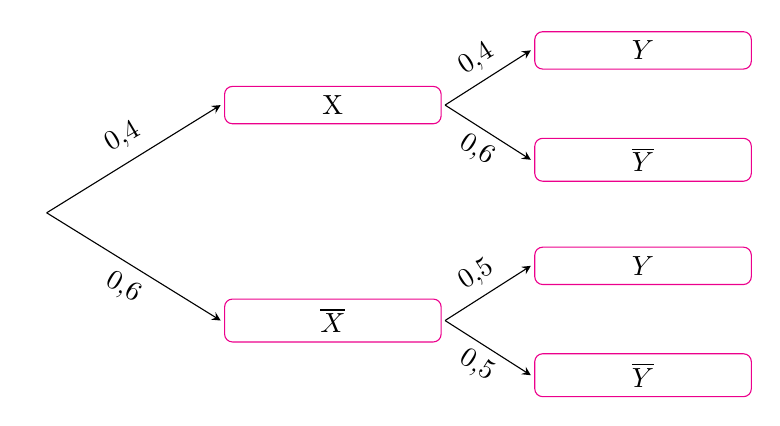
\begin{tikzpicture}
	\def\gocm{20}
	\def\gocn{10}
	\def\r{4}
	\tikzset{s/.style={outer sep=0.5 mm,draw=magenta,rectangle,minimum width=2.75cm,rounded corners=1mm}}
	\path(0,0)node(O){}++(\gocm:\r)node[s](A1){X}++(\gocn:\r)node[s](A2){$Y$};
	\path(A1)++({-\gocn}:\r)node[s](a2){$\overline{Y}$};
	\path(O)++(-\gocm:\r)node[s](B1){$\overline{X}$}++(\gocn:\r)node[s](B2){$Y$};
	\path(B1)++({-\gocn}:\r)node[s](b2){$\overline{Y}$};
	\foreach \x/\y in {
	O/A1,A1/A2,
	O/B1,B1/B2,
	A1/a2,
	B1/b2}
	\draw[-stealth](\x.east)--(\y.west);
	\path(O)--(A1.west)node[pos=0.5,above,sloped]{$0{,}4$}(O)--(B1.west)node[pos=0.5,below,sloped]{$0{,}6$}(B1.east)--(B2.west)node[pos=0.5,above,sloped]{$0{,}5$}(A1.east)--(A2.west)node[pos=0.5,above,sloped]{$0{,}4$}
	(A1.east)--(a2.west)node[pos=0.5,below,sloped]{$0{,}6$}
	(B1.east)--(b2.west)node[pos=0.5,below,sloped]{$0{,}5$};
	\end{tikzpicture}
	\end{center}
	Khi đó $\mathrm{P}(B)=\mathrm{P}(X\overline{Y})+\mathrm{P}(\overline{X}Y)=0{,}4\cdot 0{,}6+0{,}6\cdot 0{,}5=0{,}54$.
	}
\end{ex}
\begin{ex}%[2D6H1-2] 
	Cho hai biến cố $A$, $B$ có $P(A)=0{,}51$; $P(B)=0{,}2$; $P(A | B)=0{,}8$. Tính $P(B | A)$, làm tròn kết quả đến hàng phần trăm.
	\shortans{$0{,}31$}
	\loigiai{
	Ta có
	\begin{eqnarray*}
	&&P(A | B)=0{,}8\Leftrightarrow \dfrac{P(A\cap B)}{P(B)}=0{,}8\\
	&\Leftrightarrow& P(A \cap B)=0{,}8\cdot P(B)=0{,}8\cdot 0{,}2=0{,}16\\
	&\Rightarrow& P(B|A)=\dfrac{P(A\cap B)}{P(A)}=\dfrac{0{,}16}{0{,}51} \approx 0{,}31.
	\end{eqnarray*}
	}
\end{ex}
\begin{ex}%[2D6H1-2] 
	Cho hai biến cố $A$, $B$ có $P(A)=0{,}8$; $P(B)=0{,}5$; $P(A \cap B)=0{,}2$. Tính xác suất biến cố $B$ không xảy ra với điều kiện biến cố $A$ xảy ra.
	\shortans{$0{,}75$}
	\loigiai{
	Xác suất biến cố $B$ không xảy ra với điều kiện biến cố $A$ xảy ra là
	$$P(\overline{B} |A)=\dfrac{P(A\overline{B})}{P(A)}=\dfrac{P(A)-P(A\cap B)}{P(A)}=\dfrac{3}{4}=0{,}75.$$
	}
\end{ex}
\begin{ex}%[2D6V1-4] 
	Gieo một con xúc xắc cân đối và đồng chất hai lần. Tính xác suất để tổng số chấm xuất hiện trong hai lần gieo nhỏ hơn $8$. Biết rằng con lần gieo thứ nhất xuất hiện mặt $4$ chấm.
	\shortans{$0{,}5$}
	\loigiai{
	Xét các biến cố:\\
	$A$: "Lần thứ nhất xuất hiện mặt 4 chấm."\\
	$B$: "Tổng số chấm trong hai lần gieo nhỏ hơn $8$."\\
	Khi đó $$A=\{(4;1), (4;2), (4;3), (4;4), (4;5), (4;6)\};$$
	$$A\cap B= \{(4;1), (4;2), (4;3)\}.$$
	Suy ra $n(A)=6$ và $n(A\cap B)=3$.\\
	Vậy xác suất để tổng số chấm xuất hiện trong hai lần gieo bằng 6, biết rằng con lần gieo thứ nhất xuất hiện mặt 4 chấm là
	$$P(B|A)=\dfrac{n(A\cap B)}{n(A)}=\dfrac{3}{6}=0{,}5.$$
	}
\end{ex}
\begin{ex}%[2D6V1-4] 
	Một công ty bảo hiểm nhận thấy có $56 \%$ số người mua bảo hiểm sức khỏe là phụ nữ và có $42 \%$ số người mua bảo hiểm sức khỏe là phụ nữ trên 50 tuổi. Tính tỉ lệ người trên $50$ tuổi trong số những người phụ nữ mua bảo hiểm sức khỏe.
	\shortans{ $0{,}75$}
	\loigiai{
	Xét các biến cố:\\
	A: "Người mua bảo hiểm sức khỏe là phụ nữ."\\
	B: "Người mua bảo hiểm sức khỏe là phụ nữ trên $50$ tuổi."\\
	Khi đó $P(A)=0{,}56$ và $P(A \cap B)=0{,}42$.\\
	Xác suất người mua bảo hiểmTỉ lệ người trên $45$ tuổi trong số những người phụ nữ mua bảo hiểm sức khỏe là
	$$P(B|A)=\dfrac{P(A\cap B)}{P(A)}=\dfrac{0{,}42}{0{,}56}=0{,}75.$$}
\end{ex}
\begin{ex}%[2D6C1-4] 
	Tại một khu phố có $100$ căn nhà, trong đó có $40$ căn nhà gắn biển số lẻ. Biết rằng có $25$ căn nhà gắn biển số lẻ và $15$ nhà gắn biển số chẵn có ô tô. Chọn ngẫu nhiên một nhà trong khu phố đó. Tính xác suất nhà được chọn gắn biển số lẻ, biết rằng nhà đó không có ô tô.
	\shortans{$0{,}25$}
	\loigiai{
	Xét các biến cố:\\
	$A$: "Nhà được chọn gắn số lẻ."\\
	$B$: "Nhà được chọn có ô tô."\\
	Khi đó xác suất nhà được chọn gắn biển số lẻ, biết rằng nhà đó không có ô tô, là $P(A | \overline{B})$.\\
	Số căn nhà gắn số lẻ và không có ô tô là $n(A\cap \overline{B})=40-25=15$.\\
	Số căn nhà không có ô tô là $n(\overline{B})=100-(25+15)=60$.\\
	Ta có
	$$P(A | \overline{B})=\dfrac{n(A\cap \overline{B})}{n(\overline{B})}=0{,}25.$$
	}
\end{ex}
\begin{ex}%[2D6C1-4] 
	Kết quả một cuộc khảo sát các vụ tai nạn giao thông ô tô về mối quan hệ giữa việc thắt dây an toàn của người lái xe khi xảy ra tai nạn giao thông và nguy cơ tử vong của người lái xe khi xảy ra tai nạn giao thông cho thấy:
	\begin{itemize}
	\item Tỉ lệ người lái xe tử vong khi xảy ra tai nạn giao thông là $0{,4}\%$.
	\item Tỉ lệ người lái xe không thắt dây an toàn giao thông khi xảy ra tai nạn giao thông là $28 \%$.
	\item Tỉ lệ người lái xe tử vong khi xảy ra tai nạn giao thông trong trường hợp không thắt dây an toàn là $0{,}3 \%$.
	\end{itemize}
	Hỏi theo kết quả khảo sát trên, việc thắt dây an toàn của người lái xe ô tô sẽ làm giảm khả năng tử vong là bao nhiêu lần? (làm tròn đến hàng phần mười).
	\shortans{$7{,}7$}
	\loigiai{
	Chọn ngẫu nhiên một một vụ tai nạn giao thông của cuộc khảo sát trên. Xét các biến cố:\\
	$A$: "Người lái xe đó tử vong khi xảy ra tai nạn giao thông."\\
	$B$: "Người lái xe đó không thắt dây an toàn khi xảy ra tai nạn giao thông."\\
	Ta có $P(A)= 0{,4}\%$; $P(B)= 28\%$; $P(A\cap B)=0{,}3\%$.\\
	Xác suất người lái xe đó tử vong khi xảy ra tai nạn giao thông trong trường hợp không thắt dây an toàn là
	$$P(A|B)=\dfrac{P(A\cap B)}{P(B)}=\dfrac{3}{280}.$$
	Xác suất người lái xe đó có thắt dây an toàn giao thông là $P(\overline{B})=72\%$.\\
	Xác suất người lái xe đó tử vong khi xảy ra tai nạn giao thông trong trường hợp có thắt dây an toàn là
	$$P(A|\overline{B})=\dfrac{P(A\cap \overline{B})}{P(\overline{B})}=\dfrac{P(A)-P(A\cap B)}{P(\overline{B}}=\dfrac{1}{720}.$$
	Ta có
	$$\dfrac{P(A|B)}{P(A|\overline{B})}=\dfrac{54}{7}\approx7{,}7.$$
	Vậy theo khảo sát trên, việc thắt dây an toàn của người lái xe ô tô sẽ làm giảm khả năng tử vong khoảng $7{,}7$ lần.
	}
\end{ex}
\Closesolutionfile{ans}
\indapan{6}{ans/ans-2-B18-KQ}